\chapter{System Design}
\label{chap:design}

To mitigate cross-app tracking via HyTrack, we introduce a developer-defined policy mechanism enforced by cryptographically secured capability tokens that govern cookie sharing and isolation on a per-app basis.  
This chapter describes the design of this capability-based approach, the structure of the capability tokens, their enforcement model, and the overall system flow between the installer, app, browser, and web servers.

\section{Design Overview}
Our system builds on the concept of capabilities -- unforgeable tokens that grant their holder specific rights to access a resource.
Unlike traditional access control lists (ACLs), capabilities enable a decentralized and fine-grained access model, as the right to perform an operation is encoded directly within the token rather than managed by a central authority.  
This means the browser can enforce cookie access based on the capabilities presented by the app, without maintaining a global permission mapping of app identities to cookies.

Byetrack applies this principle to browser state management: cookies are encapsulated within capability tokens that specify how and under which conditions they can be accessed or stored.  
The browser acts as a Policy Enforcement Point (PEP), while the app, guided by a developer-provided policy, receives only the capabilities necessary for its legitimate functionality.

\section{Capability Token Structure}
Each capability token encodes metadata defining the scope and permissions associated with a cookie.  
The following fields form the basis of our design:

\begin{itemize}
  \item \textbf{Cookie Name and Value:} Contain the actual cookie data managed by the browser.
  \item \textbf{Signature:} Ensures the capability was issued by the browser and has not been modified.
  \item \textbf{Package Name:} Identifies the app that owns the capability.  
    This prevents implicit delegation—without it, a receiving app could reuse capabilities issued to another app.
  \item \textbf{Domain:} Specifies the target web server.  
    The browser enforces that cookies are only valid for this domain, preventing malicious libraries from reusing capabilities to store untrusted cookies in the global jar.
  \item \textbf{App Version Number:} Allows the browser to detect outdated tokens after app updates.  
    Whenever the app is updated, the installer retransmits the policy so the browser can issue new capabilities consistent with the new version.
  \item \textbf{Rights:} Define the permitted actions—reading, writing, or both—on cookie data.  
    These rights prevent tracking libraries from exploiting browser access to extract or misuse capability contents.
  \item \textbf{Global Jar Flag:} Indicates whether the cookie belongs to the shared global jar or to the app-specific isolated jar.
\end{itemize}

\section{Capability Types}
We distinguish between \textit{final}, \textit{wildcard}, and \textit{ambient} capabilities.

\begin{itemize}
  \item \textbf{Final Capabilities:} Fully specified tokens containing explicit cookie names and values.  
    They represent concrete cookie instances and are used directly for cookie enforcement.
  \item \textbf{Wildcard Capabilities:} Partially specified tokens that omit cookie names or values.  
    They serve as templates from which final tokens are derived once cookies are received from a web server.
  \item \textbf{Ambient Capabilities:} Represent the browser’s default behavior—storing all cookies in the shared global jar.  
    These act as fallbacks when no explicit policy is provided and offer no privacy guarantees.
\end{itemize}

\section{Security and Enforcement Design}
Byetrack makes browser state access explicit, app-aware, and scoped through the following principles:

\begin{itemize}
  \item \textbf{Explicit Cookie Isolation:} Cookies are stored only if a capability for the corresponding domain exists.  
    Based on the capability’s global flag, cookies are either stored in the shared jar or returned to the app for isolated local storage.
  \item \textbf{App-Aware Browser Context:} Each capability encodes the app’s identity and version, enabling the browser to enforce per-app cookie policies and invalidate outdated tokens.
  \item \textbf{Capability-Scoped Access Control:} Third-party domains without valid capabilities cannot access shared state, thereby blocking cross-app tracking.  
    Legitimate use cases such as Single Sign-On (SSO) remain supported by granting appropriate global capabilities.
\end{itemize}

\chapter{The Threat Model}
% Describe what components are trusted/untrusted / State assumption of HyTrack again (?) and our approach

% - Attacker goals (cross-app tracking through shared cookies)
% - Attacker capabilities (can embed third-party libraries, open CT/TWA, use web storage)
% - Trusted components (browser, OS integrity, capability signing)
% - Assumptions (user installs apps intentionally; developer may misconfigure but not maliciously)
% - Out-of-scope threats (fingerprinting, malicious browsers, network-level adversaries)

%\section{The Threat Model}

The developer of an Android application unknowingly includes a third-party library that uses the HyTrack technique for their own purposes, such as advertising.
We want to prevent this library from tracking the apps user across multiple apps and empower the app developer to use any third-party library without risking user privacy in regards to cross-app tracking via HyTrack.

For this, we assume that the app developer is not malicious and does not intend to violate user privacy. 
Otherwise, developers could simply choose to omit using our mitigation framework and directly use the HyTrack library on their will.

A trusted component is the installer. Next to installing the app, it also extracts the app's policy and hands it of to the (trusted) browser, the Polcy Enforcement Point (PEP).
The browser initially generates the capability tokens according to the app's policy and sends them to the app, which stores them in private storage.

As the tracking library is included in the app, it has the same permissions as the app itsef, which means it can include arbitrary code, for example attempt to modify tokens or policies.
Additionally, we have to assume collaboration between the tracking library and other apps to share stored tokens and meta data of the mitigation framework.
Attemps such as sending policy to their own benefit and thus circumventing the mitigation are also possible.

As we hook our defense in the androidx browser library, any developer that wants to use the malicous tracking library -- or any other library that relies on Custom Tabs or Trusted Web Activities -- automatically uses our mitigatin framework. Thus, the developer cannot choose to omit the mitigation, but still disable it by not giving a policy at all.
Therefore, only the androidx browser library needs to be updated, instead of relying on the developer to additionally include the mitigation library, which could be forgotten or omitted intentionally. %TODO cite research here


\section{Methodology}
\begin{figure}[h!]
  \centering
  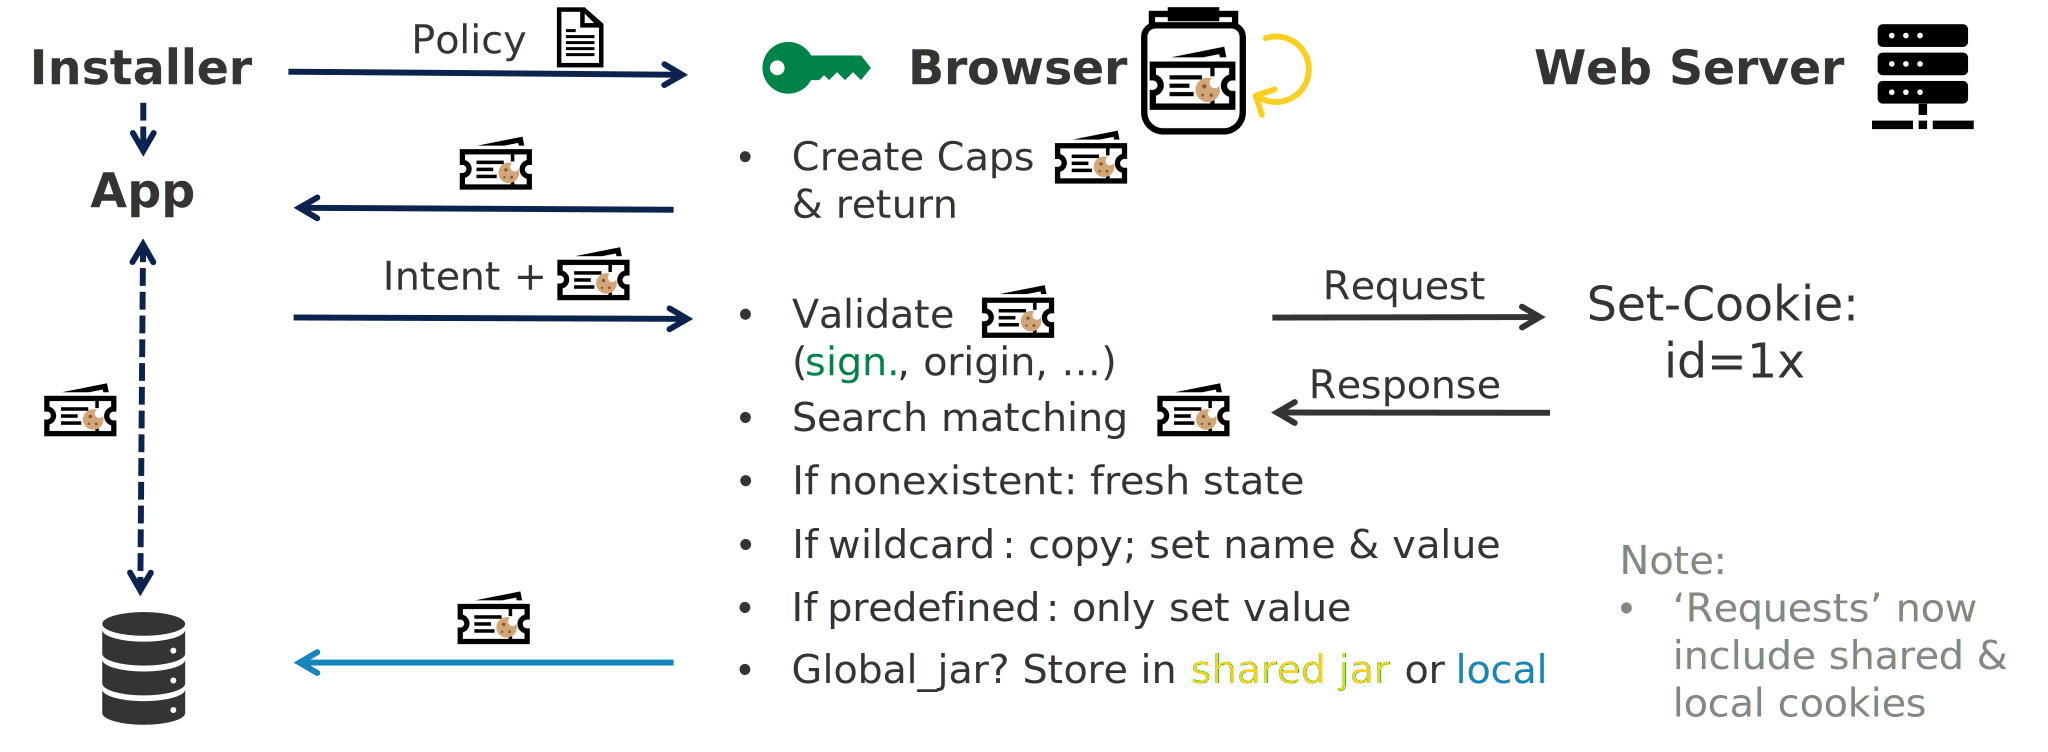
\includegraphics[width=0.9\textwidth]{ByeTrack_Flow.pdf}
  \caption{High-level overview of the Byetrack flow between installer, app, browser, and web servers.}
  \label{fig:byetrack_overview}
\end{figure}

\subsection{Developer Policy Flow}
Developers define a JSON policy that specifies which domains may share browser state and, optionally, which cookies are expected from each domain.  
This allows granular control beyond simple trusted/untrusted domain distinctions -- for example, isolating third-party cookies while permitting integration with a developer’s own authentication domain.

If no policy is provided, the browser falls back to ambient mode, where all cookies are stored in the shared jar for backwards compatibility.

\subsection{Capability Initialization}
During app installation, the installer extracts and transmits the policy to the browser.  
Before issuing any capability tokens, the browser validates and sanitizes the policy to ensure minimal privilege, removing conflicting or ambiguous entries.  

From the sanitized policy, the browser generates capability tokens as follows:
\begin{itemize}
  \item For predefined cookie entries, the browser creates corresponding predefined capability tokens.
  \item For domain-level entries, the browser issues wildcard capabilities, marking them as global or private based on the policy.
  \item If no policy is provided, a single ambient capability is issued, reverting to the default shared-cookie behavior.
\end{itemize}

Each token is signed and encrypted before being sent to the app, which stores wildcard and final tokens in private storage for later use.  
When the app is updated, the installer retransmits the policy so that the browser can reissue capabilities consistent with the new app version.

\subsection{App–Browser Interaction}
When an app opens a URL through a Custom Tab (CT) or Trusted Web Activity (TWA), the stored wildcard and (initially empty) final tokens are attached to the intent that launches the browser.  
Upon receipt, the browser decrypts and validates each token by checking its signature, package name, version number, and target domain.  
Invalid tokens are discarded.

The browser then uses the valid capabilities to:
\begin{enumerate}[label=\arabic*.]
  \item Determine how to store cookies received from the web server.
  \item Construct cookie headers for outgoing requests.
\end{enumerate}

\paragraph{Cookie Reception.}  
For every received cookie, the browser applies the following logic (in order of priority):
\begin{enumerate}[label=\arabic*.]
  \item If the token is ambient, the cookie is stored in the global jar (default behavior).
  \item If a private predefined capability matches the cookie name, the cookie value is filled in and returned to the app for local storage.
  \item If a private wildcard capability exists, the cookie is filled in accordingly and returned to the app.
  \item If a global predefined capability matches, the cookie is stored in the shared jar.
  \item If a global wildcard capability exists, any cookie from the corresponding domain is stored in the shared jar.
  \item If no capability matches, the cookie is discarded.
\end{enumerate}

\paragraph{Cookie Transmission.}  
When constructing requests, the browser merges cookies derived from the app's valid final tokens with those from its global jar, ensuring that each request accurately reflects both app-specific and shared state according to the developer policy.

\subsection{Utility Interfaces}
To improve transparency and developer control, the browser exposes limited utility functions that allow the app to:
\begin{enumerate}[label=\arabic*)]
  \item Retrieve the names of cookies encapsulated in final capabilities.
  \item Read their corresponding values.
  \item Write or update cookie values.  
\end{enumerate}
Access to these utilities is strictly controlled through capability rights: read operations require read rights, and modifications require write rights.

\section{Design Advantages}
Beyond preventing cross-app tracking, Byetrack offers several key benefits:
\begin{enumerate}[label=B\arabic*)]
  \item \textbf{Fine-Grained Control:} Developers can precisely specify which cookies are shared or isolated.
  \item \textbf{Stateless Browser Design:} The browser remains stateless with respect to app-specific data, as apps retain and transmit their own tokens.
  \item \textbf{No Web Server Changes:} Web servers operate unmodified—the browser transparently enforces the capability model.
  \item \textbf{Backwards Compatibility:} Apps without a policy fall back to the standard shared cookie behavior, ensuring compatibility with existing systems.
\end{enumerate}

\section{Alternative Design Considerations}
An alternative architecture would delegate capability generation to the installer rather than the browser.  
This would simplify the browser's responsibilities to enforcement only, reducing its complexity and eliminating installer–browser communication for each app.  
However, it would require shared cryptographic secrets between the installer and browser, thereby enlarging the trusted computing base and attack surface.  
For these reasons, the proof-of-concept implementation designates the browser as the sole trusted component for capability generation and enforcement.
